% HiMCM 2023 Problem A --- Dandelions
% Compile from paper/:
%   pdflatex himcm_paper.tex
% Every table cell is copied from ../results/*.csv. Two geometries are
% never mixed: weekly west-edge (official Req 1) vs daily center-plant CA.
\documentclass[12pt]{article}

\usepackage[margin=1in]{geometry}
\usepackage{amsmath,amssymb}
\usepackage{booktabs}
\usepackage{graphicx}
\usepackage{caption}
\usepackage{setspace}
\usepackage{array}
\usepackage[hidelinks]{hyperref}

\graphicspath{{../paper_figures/}{paper_figures/}{./}}
\hypersetup{
  pdftitle={HiMCM 2023 Problem A: Dandelions},
  pdfauthor={GoHiMCM 2023 A study team}
}

\newcommand{\TeamNumber}{GoHiMCM}
\newcommand{\vt}{v_{t}}
\newcommand{\smi}{\theta}

\pagestyle{myheadings}
\markright{\TeamNumber \hfill HiMCM 2023 Problem A \hfill}

\title{\textbf{Pappus Plumes on One Hectare: Convolution, Fisher--KPP, and a Lawn Pareto}\\[0.4em]
\large HiMCM 2023 Problem A --- Team \TeamNumber}
\author{}
\date{}

\begin{document}
\maketitle
\thispagestyle{empty}

\noindent
A one-page numerical digest is \texttt{summary\_sheet.tex}.
The community letter is \texttt{hoa\_community\_statement.tex}.
This paper does not reuse stale cells from an earlier weekly run
(cover $0.2097$, $I_{\mathrm{TAROF}}=0$): the locked CSVs now in
\texttt{results/} are the only source.

\tableofcontents
\newpage

\section{Problem and two geometries}
Official Req~1 asks how far \emph{Taraxacum officinale} spreads from
\textbf{one puffball-stage plant adjacent to a $100\times 100\,\mathrm{m}$ plot}
at months $1,2,3,6,12$ under temperate, arid, and tropical forcing.
Official Req~2 is a locked SAW impact factor against two other invaders---not
a mowing essay.
Course extensions add a weekly mowing Pareto, a daily center-plant
cellular automaton (CA), a Fisher--KPP slope check, and an HOA note.

We keep two universes separate.
\begin{itemize}
  \item \textbf{Weekly west-edge} (\texttt{engine.py}): source at
        $(-0.5,50)\,\mathrm{m}$; Lefkovitch week-step; hybrid Gaussian+WALD
        kernel; checkpoints in \texttt{monthly\_metrics.csv}.
  \item \textbf{Daily center CA} (\texttt{grid\_engine.py}): $t=0$ is one
        adult at cell $(50,50)$; $K_{\mathrm{cell}}=15$; 25-day seedlings;
        $\mathrm{convolve2d}(180A,\mathcal{K}_t)$; checkpoints in
        \texttt{monthly\_population\_metrics.csv}.
\end{itemize}
A temperate month-12 cover of $0.4511$ (weekly) is not the daily CA's
$100\%$ occupancy. Mixing them is a two-universe error.

\section{Aerodynamic kernel}
Pappus flight uses a near-field bivariate Gaussian plus a thermal-updraft
WALD tail~\cite{katul2005}:
\begin{equation}
  K_{\mathrm{disp}}=(1-p_{\mathrm{up}})K_{\mathrm{base}}+p_{\mathrm{up}}K_{\mathrm{up}},
  \qquad
  \Phi(T,\theta)=f_T(T)\,g_\theta(\theta).
\end{equation}
The WALD along-wind law is Inverse-Gaussian
\begin{equation}
  \mu=\frac{H\bar U}{\vt},\qquad
  \lambda=\frac{\mu}{\kappa^{2}},\qquad
  f(r)=\sqrt{\frac{\lambda}{2\pi r^{3}}}
  \exp\Bigl(-\frac{\lambda(r-\mu)^{2}}{2\mu^{2} r}\Bigr).
\end{equation}
Engine constants live in \texttt{data/parameters/biophysics.json}
($H=0.35\,\mathrm{m}$, $\vt=0.32\,\mathrm{m\,s}^{-1}$, $\kappa=0.40$).
The hybrid module uses $H_0=0.25\,\mathrm{m}$, $\vt=0.28\,\mathrm{m\,s}^{-1}$,
$p_{\mathrm{up}}=0.03$, $H_{\mathrm{up}}=12.5\,\mathrm{m}$ and does not
overwrite the WALD-engine contract.
Meteorological wind maps to the downwind unit $(- \sin\theta,-\cos\theta)$.
Discrete kernels are renormalized so $\sum_{ij}K_{ij}=1$ before convolution.
There is no per-seed particle loop.

\section{Requirement 1 --- weekly hectare}
Each cell holds $(S,L,R,A)$. Climate multiplies Lefkovitch rates by
$\varphi(T,\smi)$. Canopy $R+A$ is Yoda-capped at
$K_{\mathrm{eff}}=K\,\smi^{a}$.
Bloom months: temperate $\{4,5,6,9,10\}$, arid $\{3,4,5\}$, tropical all year.
A fraction $\varepsilon=0.05$ of fence-line seeds is retained locally so an
offshore tropical easterly does not erase the plot by underflow.

Table~\ref{tab:weekly} is copied from \texttt{monthly\_metrics.csv}.
Months $1$--$3$ on the temperate west-edge run are still empty: the first
recruits appear in month~$4$ ($n_{\mathrm{plants}}=90.03$, front $6.5\,\mathrm{m}$).
Month~$6$ is a single expanding lobe (cover $0.0328$, front $13.5\,\mathrm{m}$).
Month~$12$ cover is $0.4511$ with $n_{\mathrm{plants}}=4.414\times 10^{5}$
and $n_{\mathrm{adult}}=4674$---seedlings dominate the head-count.
Arid month~$12$ cover is $0.0065$; tropical is $0.0232$ with a $10.5\,\mathrm{m}$
front. Halving temperate $\smi$ cuts month-$12$ cover from $0.4511$ to
$0.2046$ (\texttt{drought\_monthly.csv}).

\begin{table}[h]
\centering
\caption{Weekly west-edge checkpoints. Source: \texttt{monthly\_metrics.csv}.
$n_{\mathrm{plants}}=L+R+A$.}
\label{tab:weekly}
\begin{tabular}{llrrr}
\toprule
Climate & Month & Cover & $n_{\mathrm{plants}}$ & Front (m) \\
\midrule
temperate & 1 & 0.0000 & 0 & 0.0 \\
temperate & 2 & 0.0000 & 0 & 0.0 \\
temperate & 3 & 0.0000 & 0 & 0.0 \\
temperate & 6 & 0.0328 & $1.521\times 10^{4}$ & 13.5 \\
temperate & 12 & 0.4511 & $4.414\times 10^{5}$ & 99.5 \\
arid & 12 & 0.0065 & 27.92 & 13.5 \\
tropical & 12 & 0.0232 & $4.747\times 10^{4}$ & 10.5 \\
\bottomrule
\end{tabular}
\end{table}

\begin{figure}[h]
\centering
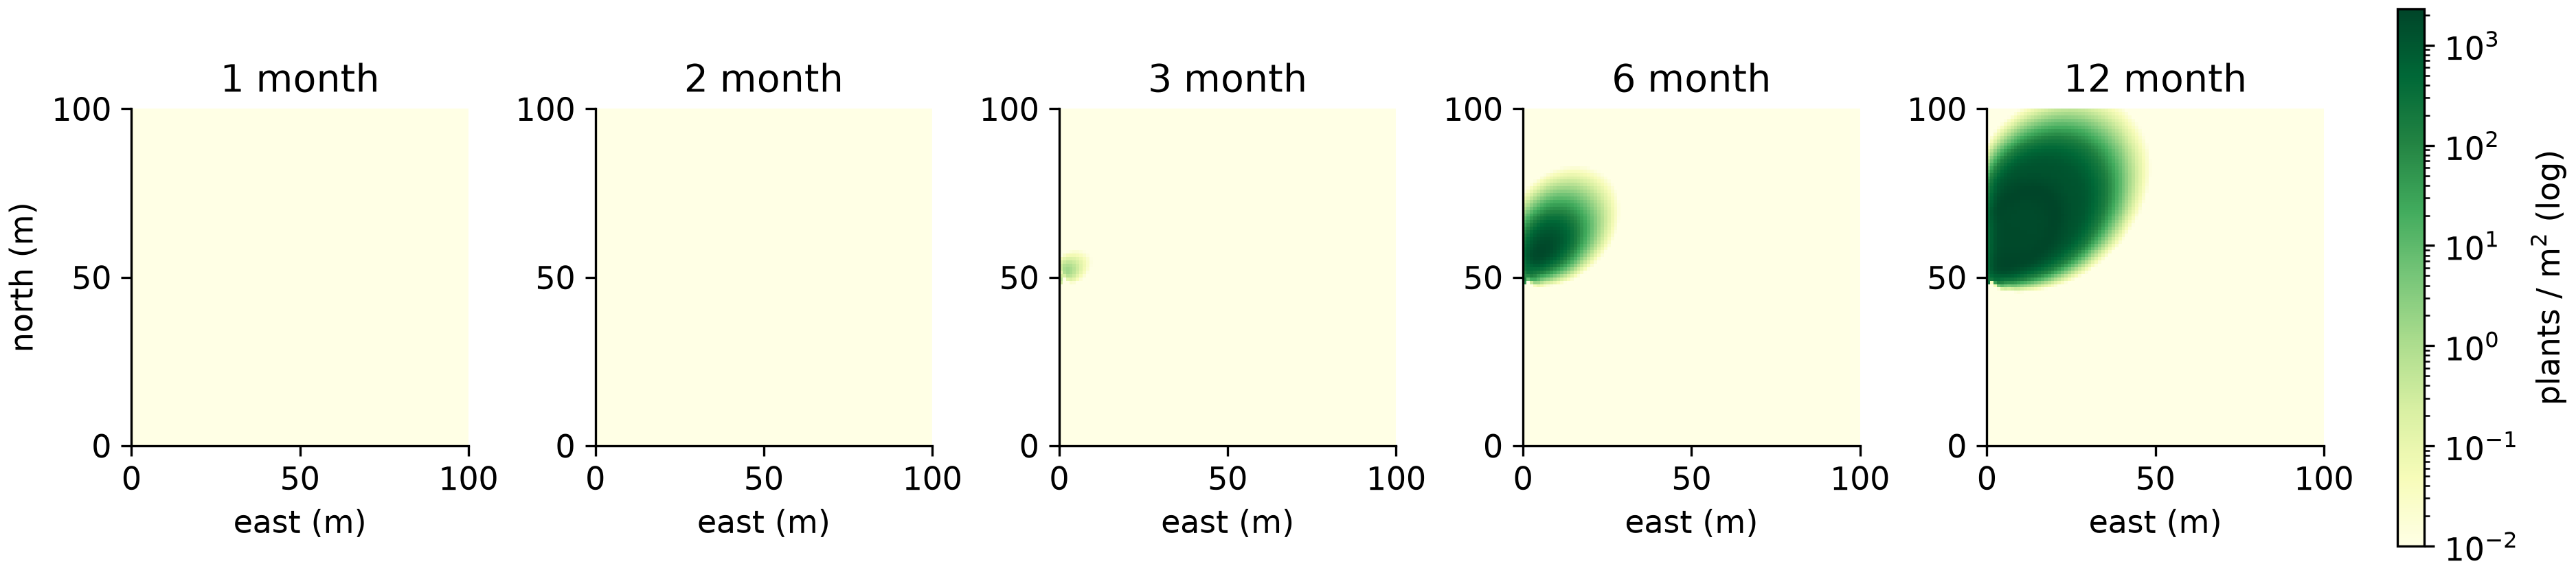
\includegraphics[width=\textwidth]{fig_heatmap_temperate.png}
\caption{Weekly temperate $L+R+A$ (log) at months $1,2,3,6,12$.
Source: \texttt{results/snapshots/temperate\_week*.npy}.}
\label{fig:heatW}
\end{figure}

\begin{figure}[h]
\centering
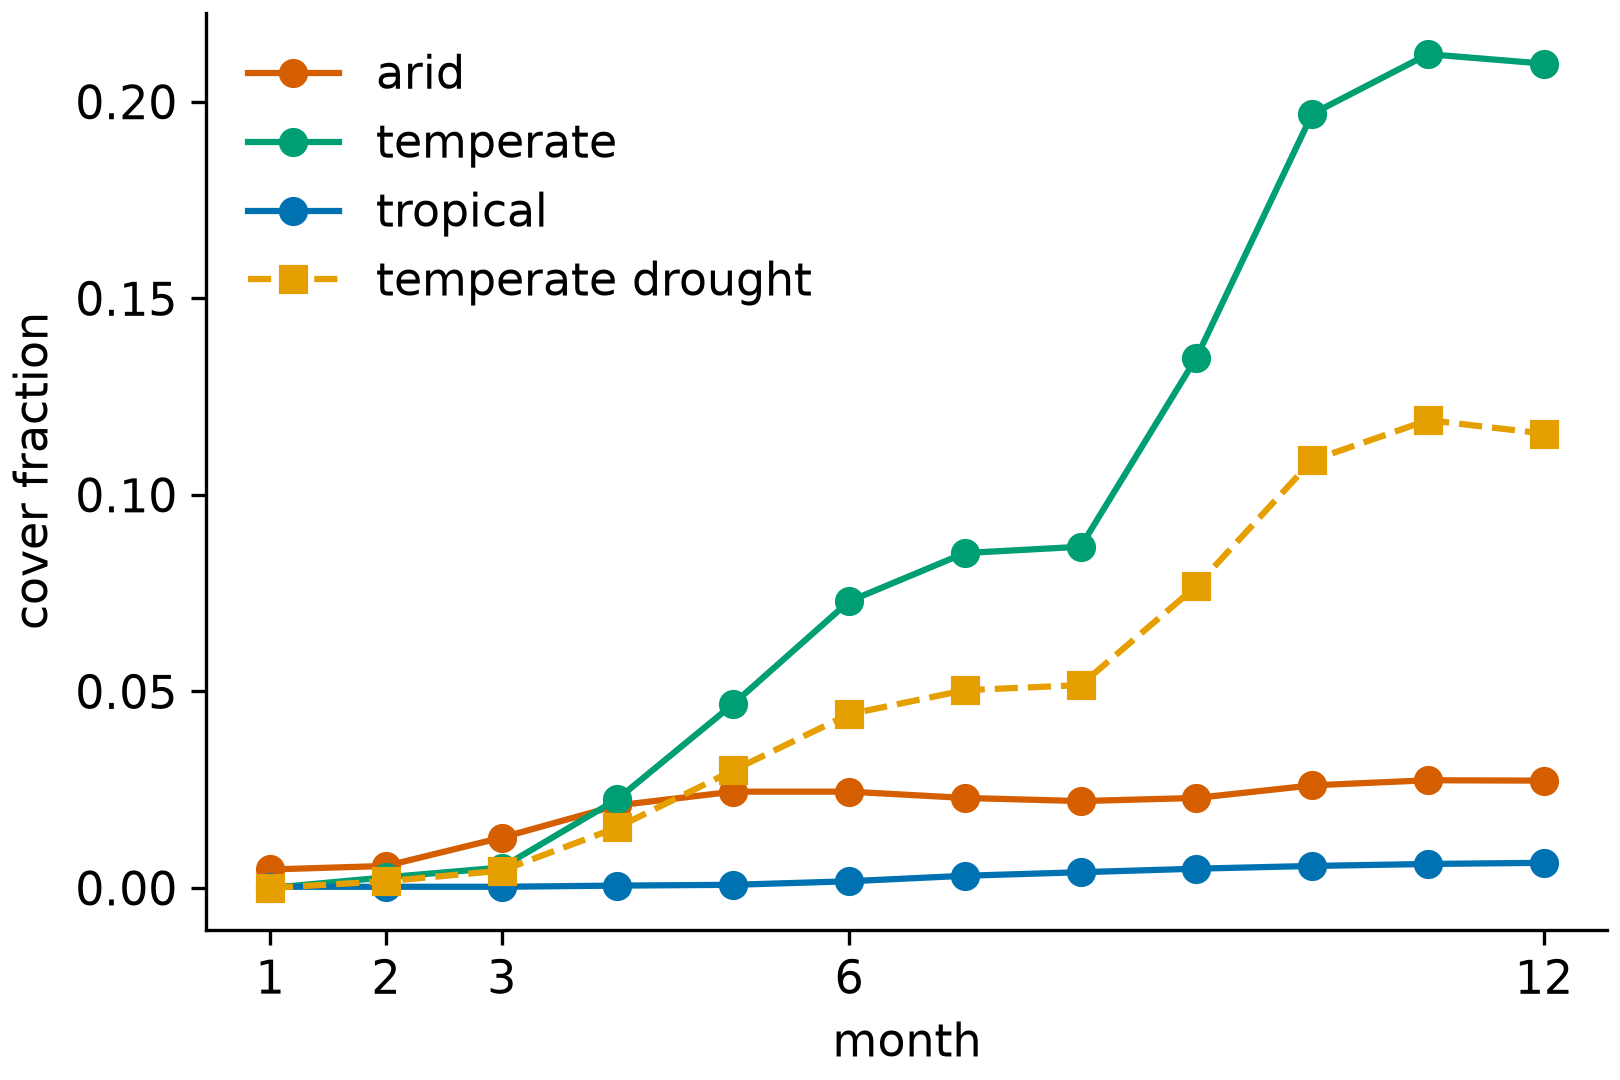
\includegraphics[width=0.72\textwidth]{fig_climate_cover.png}
\caption{Weekly cover by climate, plus temperate drought $\smi\times 0.5$
(month-12 cover $0.2046$).}
\label{fig:cover}
\end{figure}

\section{Daily center CA (companion, not Req~1 geometry)}
The daily engine starts one flowering adult at $(50,50)$, releases
$180$ seeds per adult on bloom days, and uses absorbing boundaries
(\texttt{convolve2d}, \texttt{mode=same}).
Table~\ref{tab:daily} is \texttt{monthly\_population\_metrics.csv}.
At day~$30$ the original adult is still alone ($n_{\mathrm{adult}}=0.942$,
$R_{95}=0$, cover $0.01\%$)---no new cohort yet.
Day~$60$ first shows a $5.02\,\mathrm{m}$ $R_{95}$.
Day~$90$ has $n_{\mathrm{plants}}=21.32$ and $R_{95}=7.01\,\mathrm{m}$
while adults remain $\approx 1$: the first filial plants are seedlings and
rosettes, not $214$ flowering heads.
Day~$180$ is a filled core (cover $34.73\%$, $R_{95}=46.12\,\mathrm{m}$).
Day~$365$ saturates the hectare (cover $100\%$, $R_{95}=60\,\mathrm{m}$).

\begin{table}[h]
\centering
\caption{Daily center-plant CA. Source: \texttt{monthly\_population\_metrics.csv}.}
\label{tab:daily}
\begin{tabular}{rrrrr}
\toprule
Day (month) & $n_{\mathrm{adult}}$ & $n_{\mathrm{plants}}$ & $R_{95}$ (m) & Cover \\
\midrule
30 (1) & 0.942 & 1.04 & 0.00 & $0.01\%$ \\
60 (2) & 0.888 & 3.19 & 5.02 & $0.16\%$ \\
90 (3) & 1.062 & 21.32 & 7.01 & $0.39\%$ \\
180 (6) & $4.761\times 10^{3}$ & $6.181\times 10^{5}$ & 46.12 & $34.73\%$ \\
365 (12) & $1.038\times 10^{5}$ & $2.762\times 10^{6}$ & 60.00 & $100\%$ \\
\bottomrule
\end{tabular}
\end{table}

\begin{figure}[h]
\centering
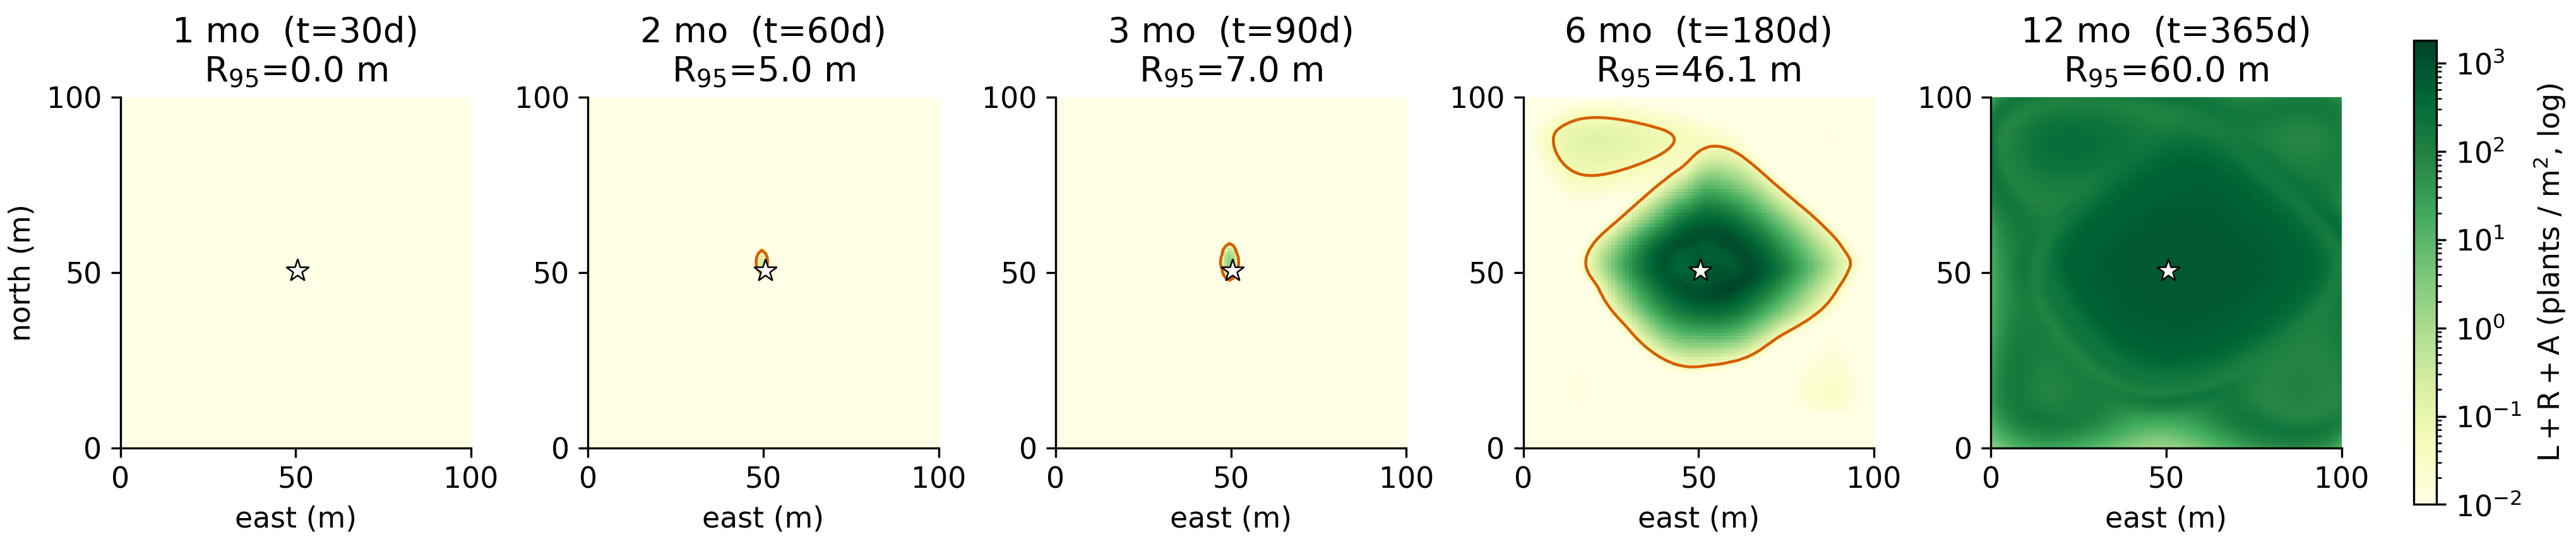
\includegraphics[width=\textwidth]{fig_spatial_spread_5stages.png}
\caption{Daily CA at days $30,60,90,180,365$, shared log scale, origin
$(50,50)$ and $0.05\,\mathrm{m}^{-2}$ front.
Source: \texttt{results/snapshots/hectare\_day*.npy}.}
\label{fig:heatD}
\end{figure}

\section{Fisher--KPP multi-scale check}
The continuum model~\cite{fisher1937,simpson2024} is
\begin{equation}
  \partial_t u = D\nabla^2 u + r u\bigl(1-u/K\bigr),
  \qquad
  c^{\ast}=2\sqrt{rD}.
\end{equation}
In two dimensions $D=M_2/(4\tau)$. With $\sigma_{\mathrm{wind}}^2:=M_2/2$
and $\tau=1\,\mathrm{d}$ this is identical to
$D=\tfrac12\sigma_{\mathrm{wind}}^2$.
Intrinsic $r=\ln\rho/\tau$ uses the Lefkovitch (weekly) or daily projection
spectral radius.
Physically admissible waves satisfy dimensionless $c\ge 2$; we report
dimensional $c^{\ast}$ and a late-time slope $c_{\mathrm{num}}$ on an
isodensity $X(t)$. We do \emph{not} set the 12-month front equal to
$52c^{\ast}$ or $365c^{\ast}$.

Weekly temperate (\texttt{kpp\_check.csv}):
$D=4.7959\,\mathrm{m}^{2}\,\mathrm{wk}^{-1}$,
$r=0.6554\,\mathrm{wk}^{-1}$,
$c^{\ast}=3.5458\,\mathrm{m\,wk}^{-1}$,
$c_{\mathrm{num}}=3.3611\,\mathrm{m\,wk}^{-1}$,
relative error $0.0521$.

Daily CA (\texttt{daily\_kpp\_check.csv}):
$D=7.2322\,\mathrm{m}^{2}\,\mathrm{d}^{-1}$,
$r=0.0842\,\mathrm{d}^{-1}$,
$c^{\ast}=1.5608\,\mathrm{m\,d}^{-1}$,
$c_{\mathrm{num}}=0.3572\,\mathrm{m\,d}^{-1}$ on days $146$--$175$
($R_{95}<42\,\mathrm{m}$), relative error $0.771$.
The large gap is expected: 25-day stage delay, seasonal bloom, and a
$50\,\mathrm{m}$ half-width absorb the pulled-front $c^{\ast}$
(Figure~\ref{fig:kpp}).

\begin{figure}[h]
\centering
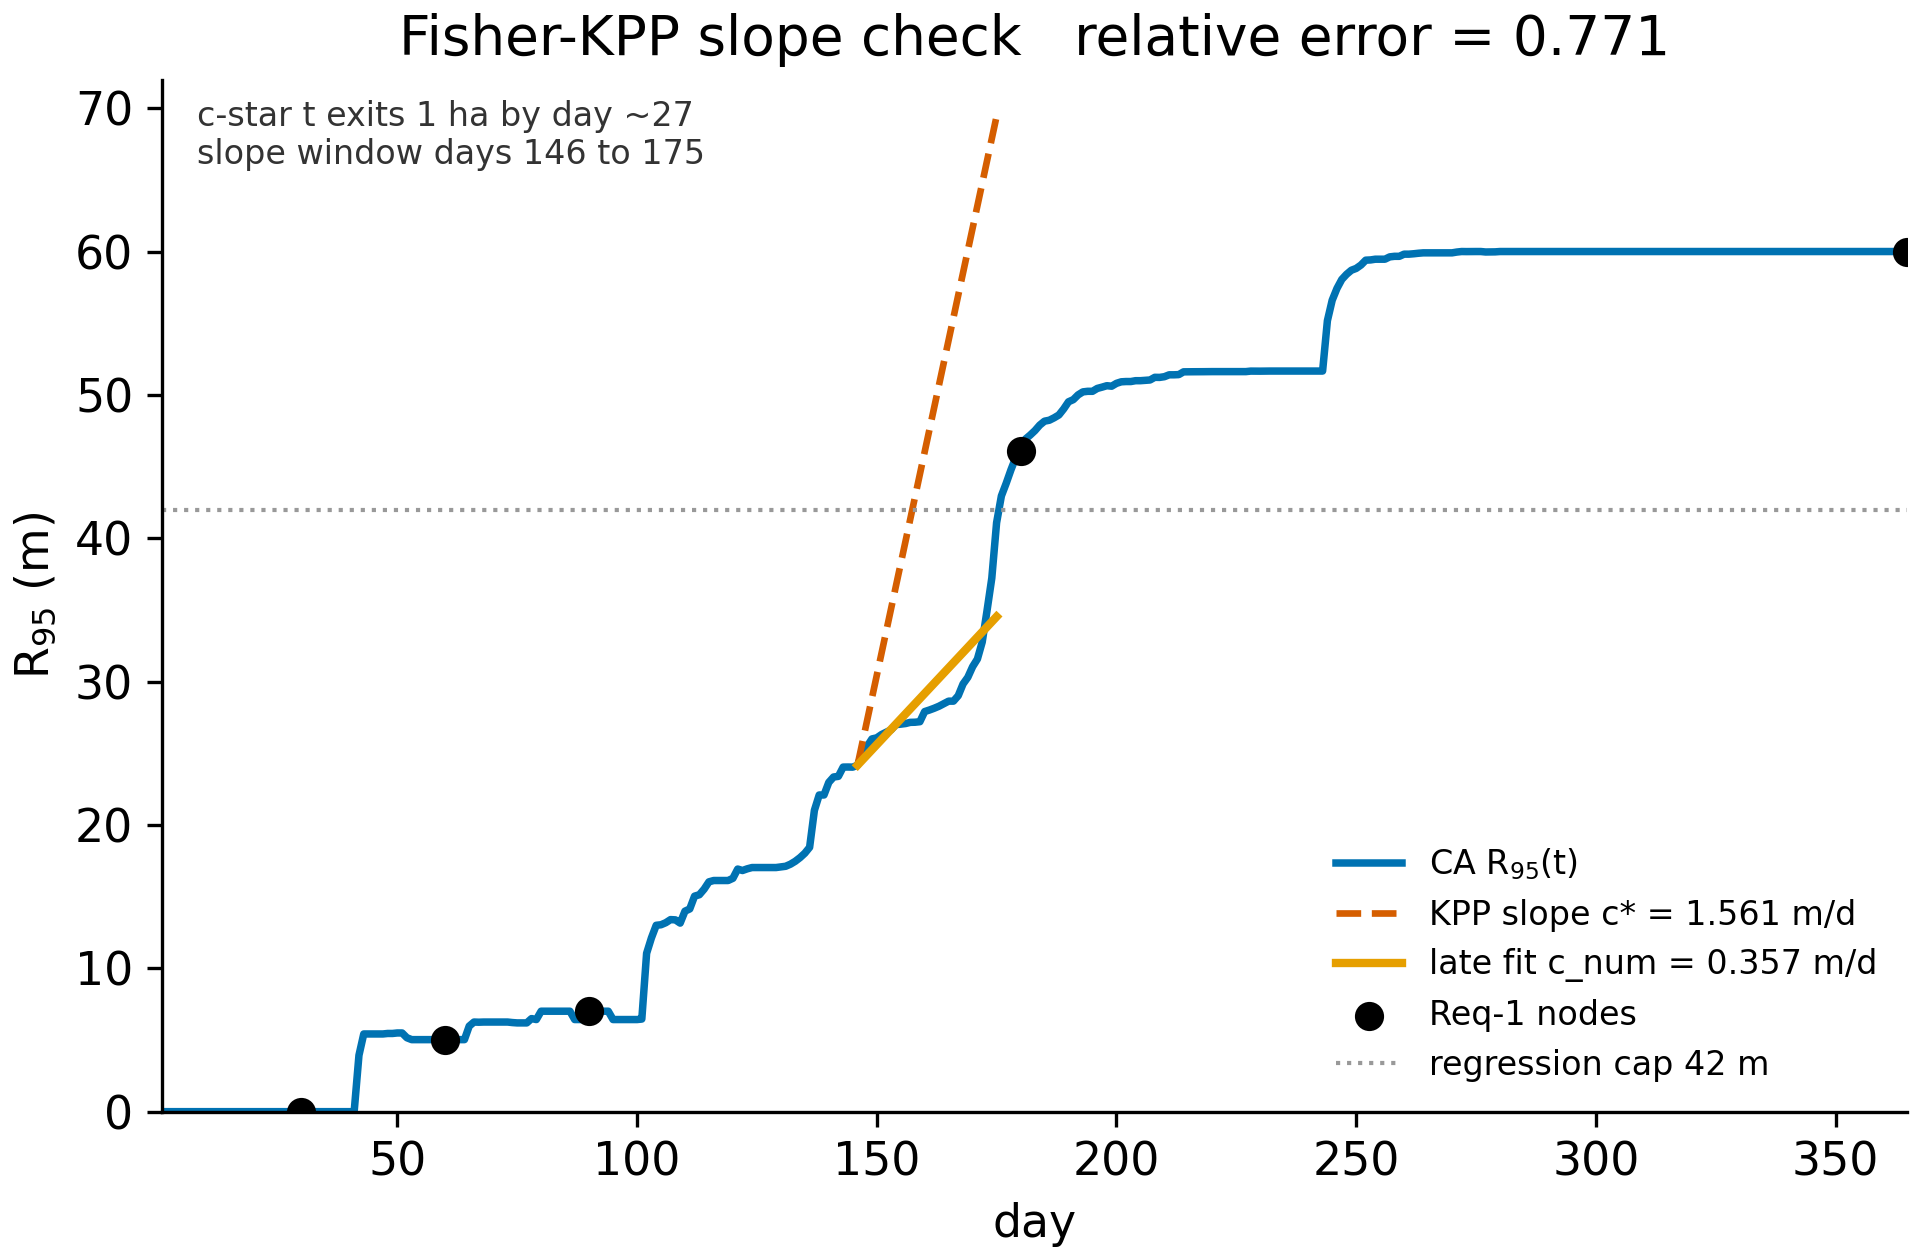
\includegraphics[width=0.78\textwidth]{fig_pde_vs_simulation_wave.png}
\caption{Daily $R_{95}(t)$ versus KPP slope on the expanding window.
Source: \texttt{daily\_front\_radius.csv}, \texttt{daily\_kpp\_check.csv}.}
\label{fig:kpp}
\end{figure}

\section{Requirement 2 --- impact factor}
Locked SAW on six 1--9 leaves, utility in the cost sense:
\begin{equation}
  I=\sum_{k\in\mathcal{B}}w_k\tilde x_k+\sum_{k\in\mathcal{C}}w_k(1-\tilde x_k).
\end{equation}
Min-max $\tilde x$ is taken only on
\{\emph{T.\ officinale}, kudzu, Japanese knotweed\}.
Dandelion spread is $1+8(1-e^{-\mathrm{cover}_{12}/0.15})=8.6046$ from the
\textbf{weekly} temperate cover $0.4511$.
Table~\ref{tab:impact} is \texttt{impact\_factors.csv}:
kudzu $I=0.9333$, knotweed $I=0.5700$, dandelion $I=0.1512$.
$I_{\mathrm{TAROF}}$ is smallest \emph{inside this three-row universe},
not a certificate that dandelion is harmless outdoors.

\begin{table}[h]
\centering
\caption{Impact $I$. Source: \texttt{impact\_factors.csv}.}
\label{tab:impact}
\begin{tabular}{llcr}
\toprule
Code & Region & Spread leaf & $I$ \\
\midrule
PUMON & SE United States & 9.00 & 0.9333 \\
REJAP & UK / NE US riparian & 8.00 & 0.5700 \\
TAROF & N.\ American lawns & 8.60 (weekly cover) & 0.1512 \\
\bottomrule
\end{tabular}
\end{table}

\section{Course control --- weekly Pareto and daily PRISMS}
\subsection{Weekly $J=(\mathrm{cover}_{12},C)$}
Relative cost $C=n_{\mathrm{mow}}(1+\eta/2)$.
Table~\ref{tab:pareto} and Figure~\ref{fig:pareto} are
\texttt{bioeconomic\_pareto.csv}.
Never-mow is $(0.4511,0)$.
Biweekly $\eta=1$ reaches cover $0.0064$ at $C=39$ and is on the front.
Weekly $\eta=1$ repeats cover $0.0064$ at $C=78$ and is dominated.

\begin{table}[h]
\centering
\caption{Selected temperate mowing points.
Source: \texttt{bioeconomic\_pareto.csv}.}
\label{tab:pareto}
\begin{tabular}{rrrrc}
\toprule
Interval (wk) & $\eta$ & Cover & $C$ & Front? \\
\midrule
0 & 0.0 & 0.4511 & 0.0 & yes \\
13 & 1.0 & 0.3834 & 6.0 & yes \\
2 & 1.0 & 0.0064 & 39.0 & yes \\
1 & 1.0 & 0.0064 & 78.0 & no \\
\bottomrule
\end{tabular}
\end{table}

\begin{figure}[h]
\centering
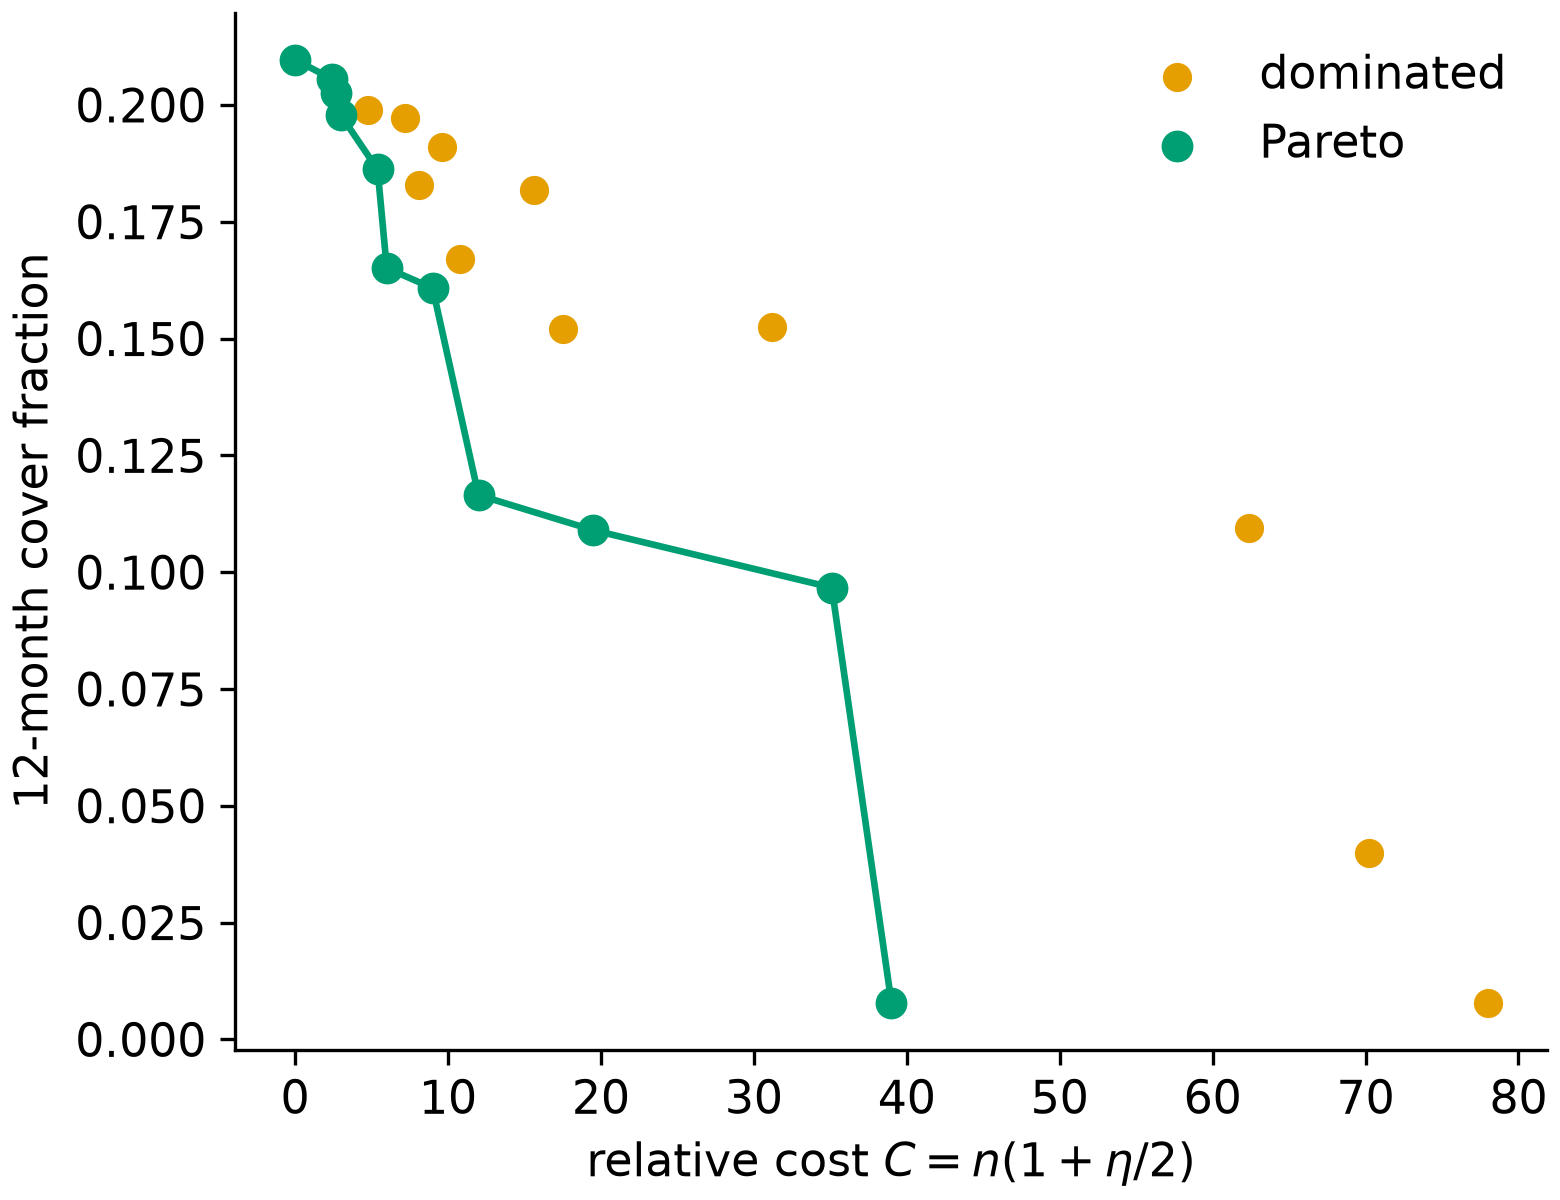
\includegraphics[width=0.72\textwidth]{fig_pareto_mowing.png}
\caption{Weekly temperate mowing front. Source: \texttt{bioeconomic\_pareto.csv}.}
\label{fig:pareto}
\end{figure}

\subsection{Daily four-strategy scores}
Benefits and costs
\begin{align}
  B_{\mathrm{eco}}&=\alpha F_{\mathrm{spring}}+\beta\,\overline{R+A},\\
  C_{\mathrm{turf}}&=\gamma\,(\mathrm{cover}_{365})^{1.3},\\
  C_{\mathrm{cost}}&=C_{\mathrm{turf}}+c_m n(1+\eta/2)+c_h n_{\mathrm{spray}}
\end{align}
are evaluated on the daily CA
(\texttt{bioeconomic\_tradeoff.csv}).
$B$ is rescaled to the wild run so $\alpha,\beta,\gamma$ stay $O(1)$
relative weights, not dollars.
Strategy~4 (PRISMS) keeps $\approx 14$ bloom days, then one low-deck cut
three days before the modeled seed pulse.

Wild: $B_{\mathrm{eco}}=1.600$, $C_{\mathrm{cost}}=1.200$, cover $100\%$,
net $+0.400$ (only non-dominated point on $(B_{\mathrm{eco}},C_{\mathrm{cost}})$).
PRISMS: $B_{\mathrm{pollinator}}=0.518$ ($51.8\%$ of wild),
$B_{\mathrm{soil}}=0.592$, $B_{\mathrm{eco}}=1.110$, one mow,
year-end cover still $100\%$,
$n_{\mathrm{plants}}$ $2.640\times 10^{6}$ versus wild $2.762\times 10^{6}$
($4.4\%$ fewer standing plants---not a $68\%$ seed cut).
Weekly mowing: cover $25.51\%$, $C_{\mathrm{cost}}=2.056$.
Herbicide: cover $68.41\%$, ten sprays, $C_{\mathrm{cost}}=1.933$.

\begin{figure}[h]
\centering
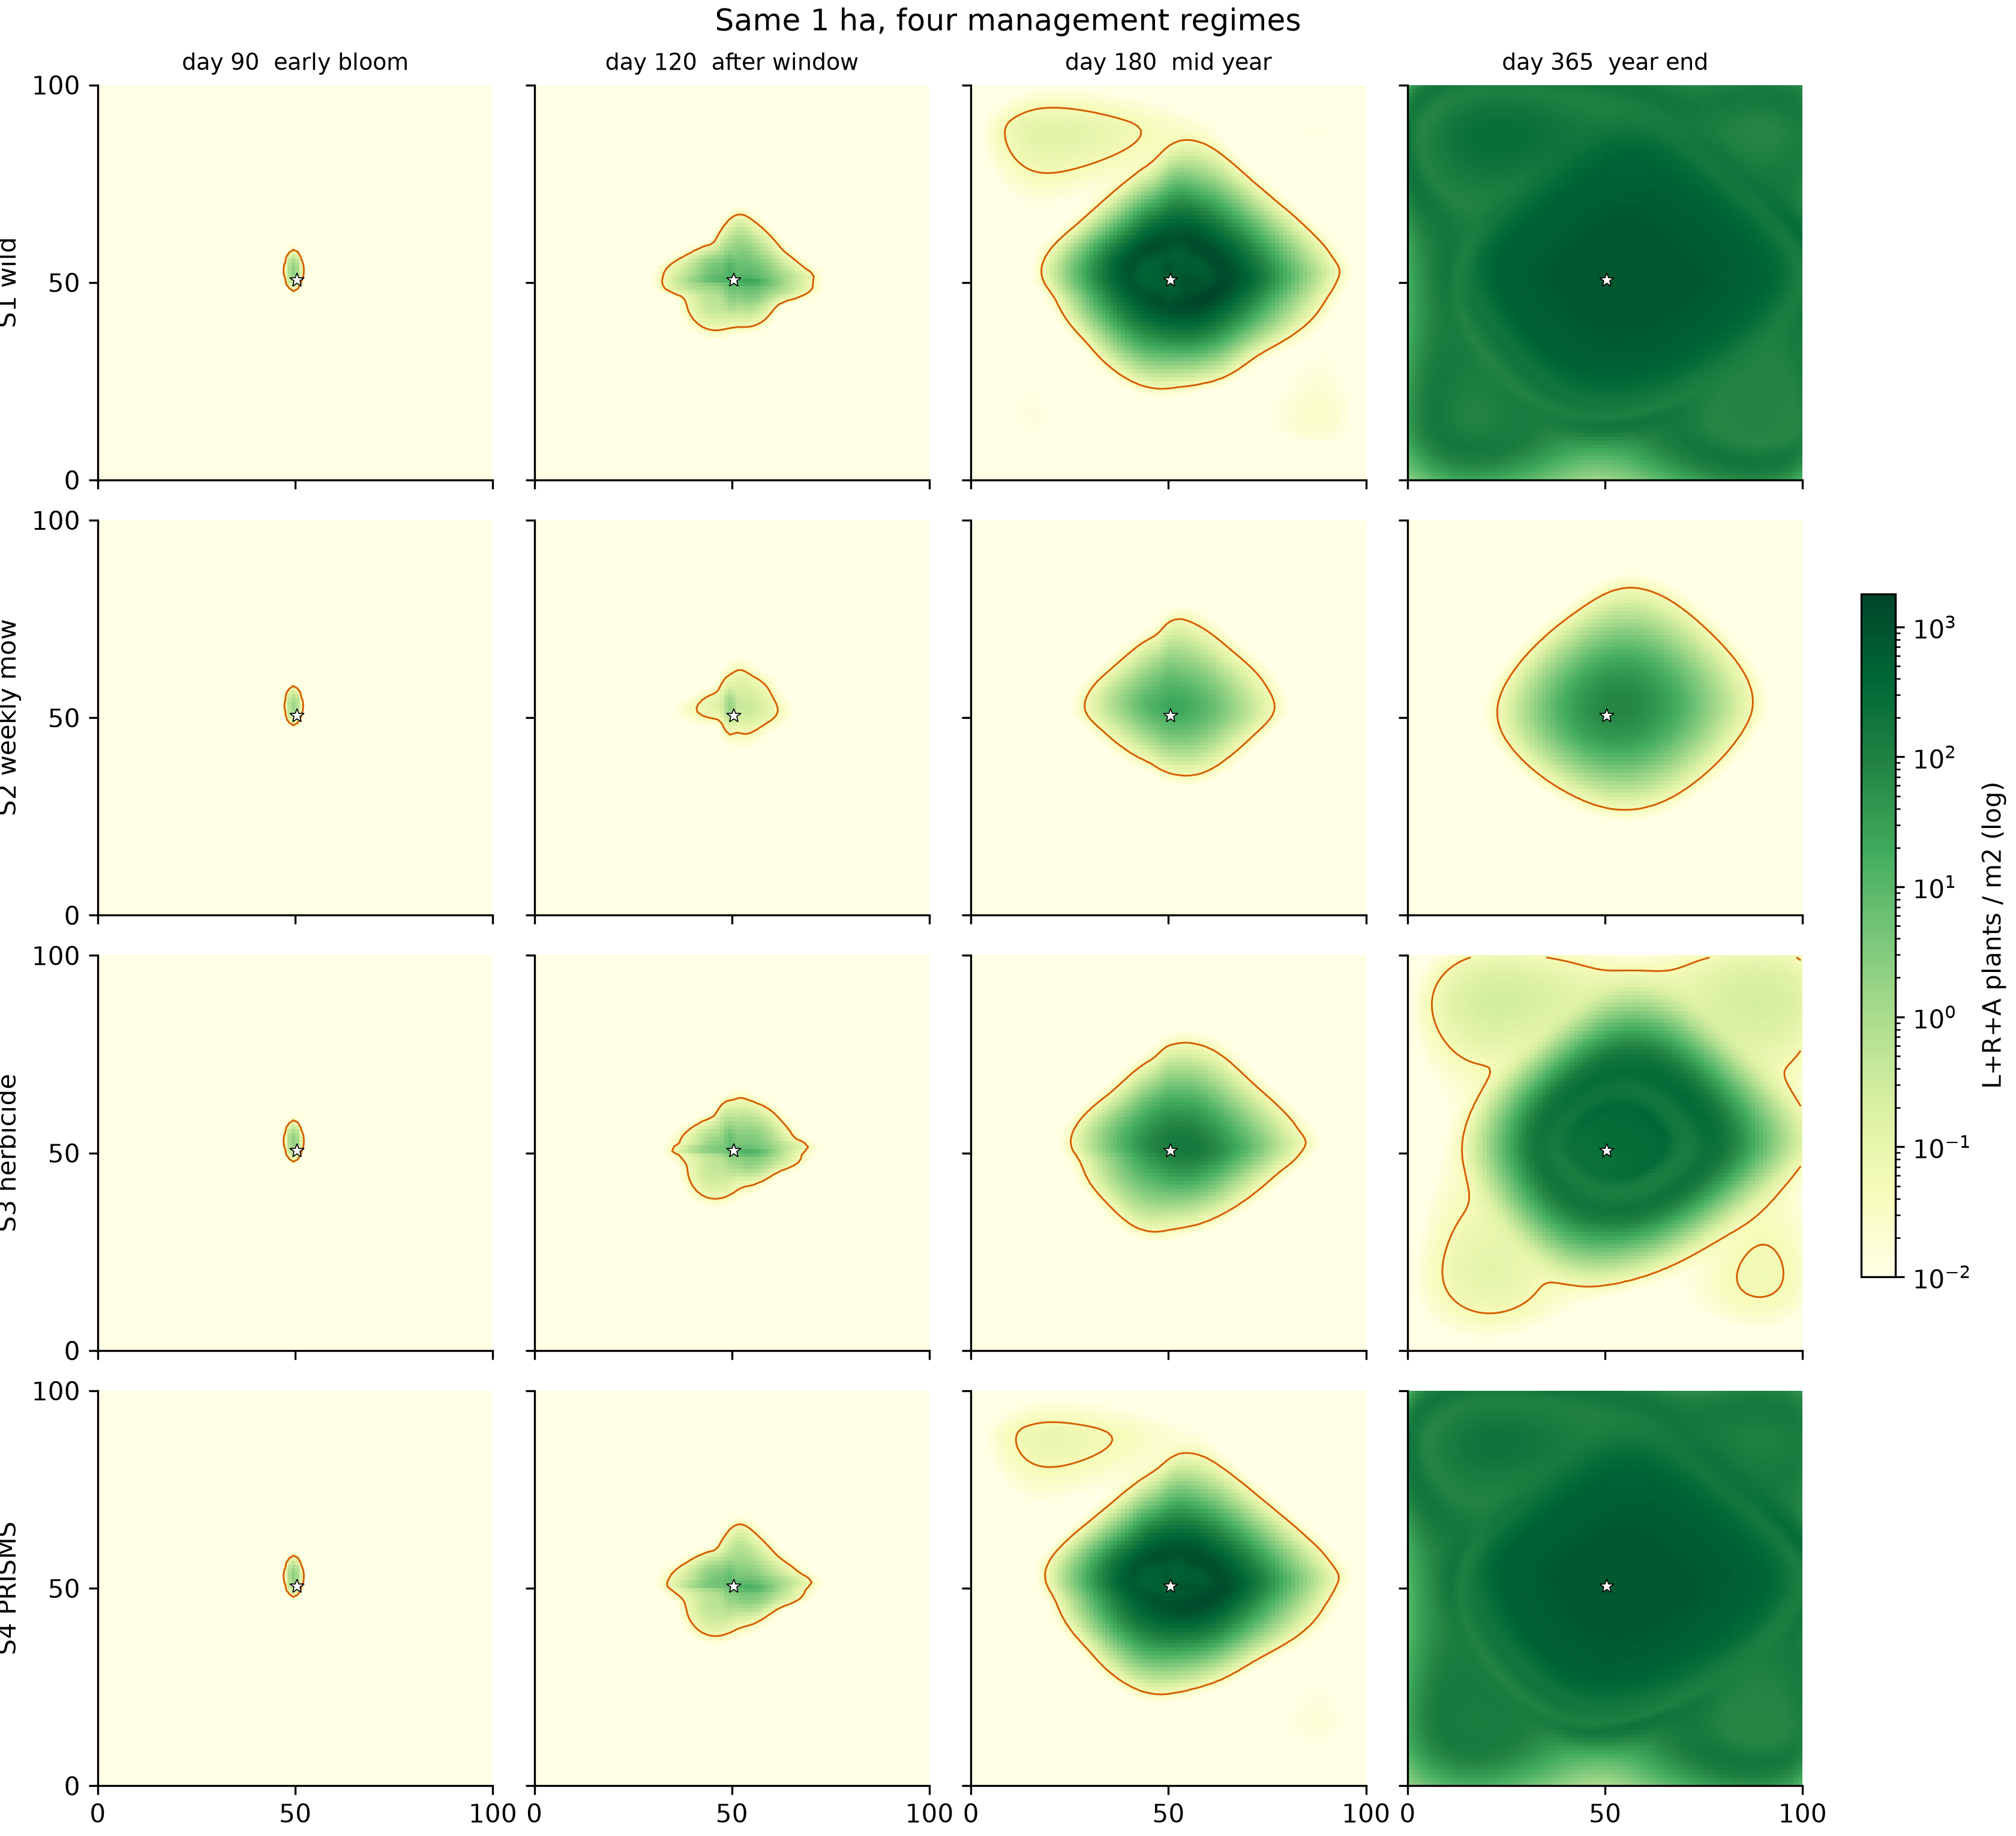
\includegraphics[width=\textwidth]{fig_strategy_spatial_effects.png}
\caption{Daily CA under four regimes at days $90,120,180,365$.
Source: \texttt{snapshots/tradeoff\_*\_day*.npy}.}
\label{fig:four}
\end{figure}

\begin{figure}[h]
\centering
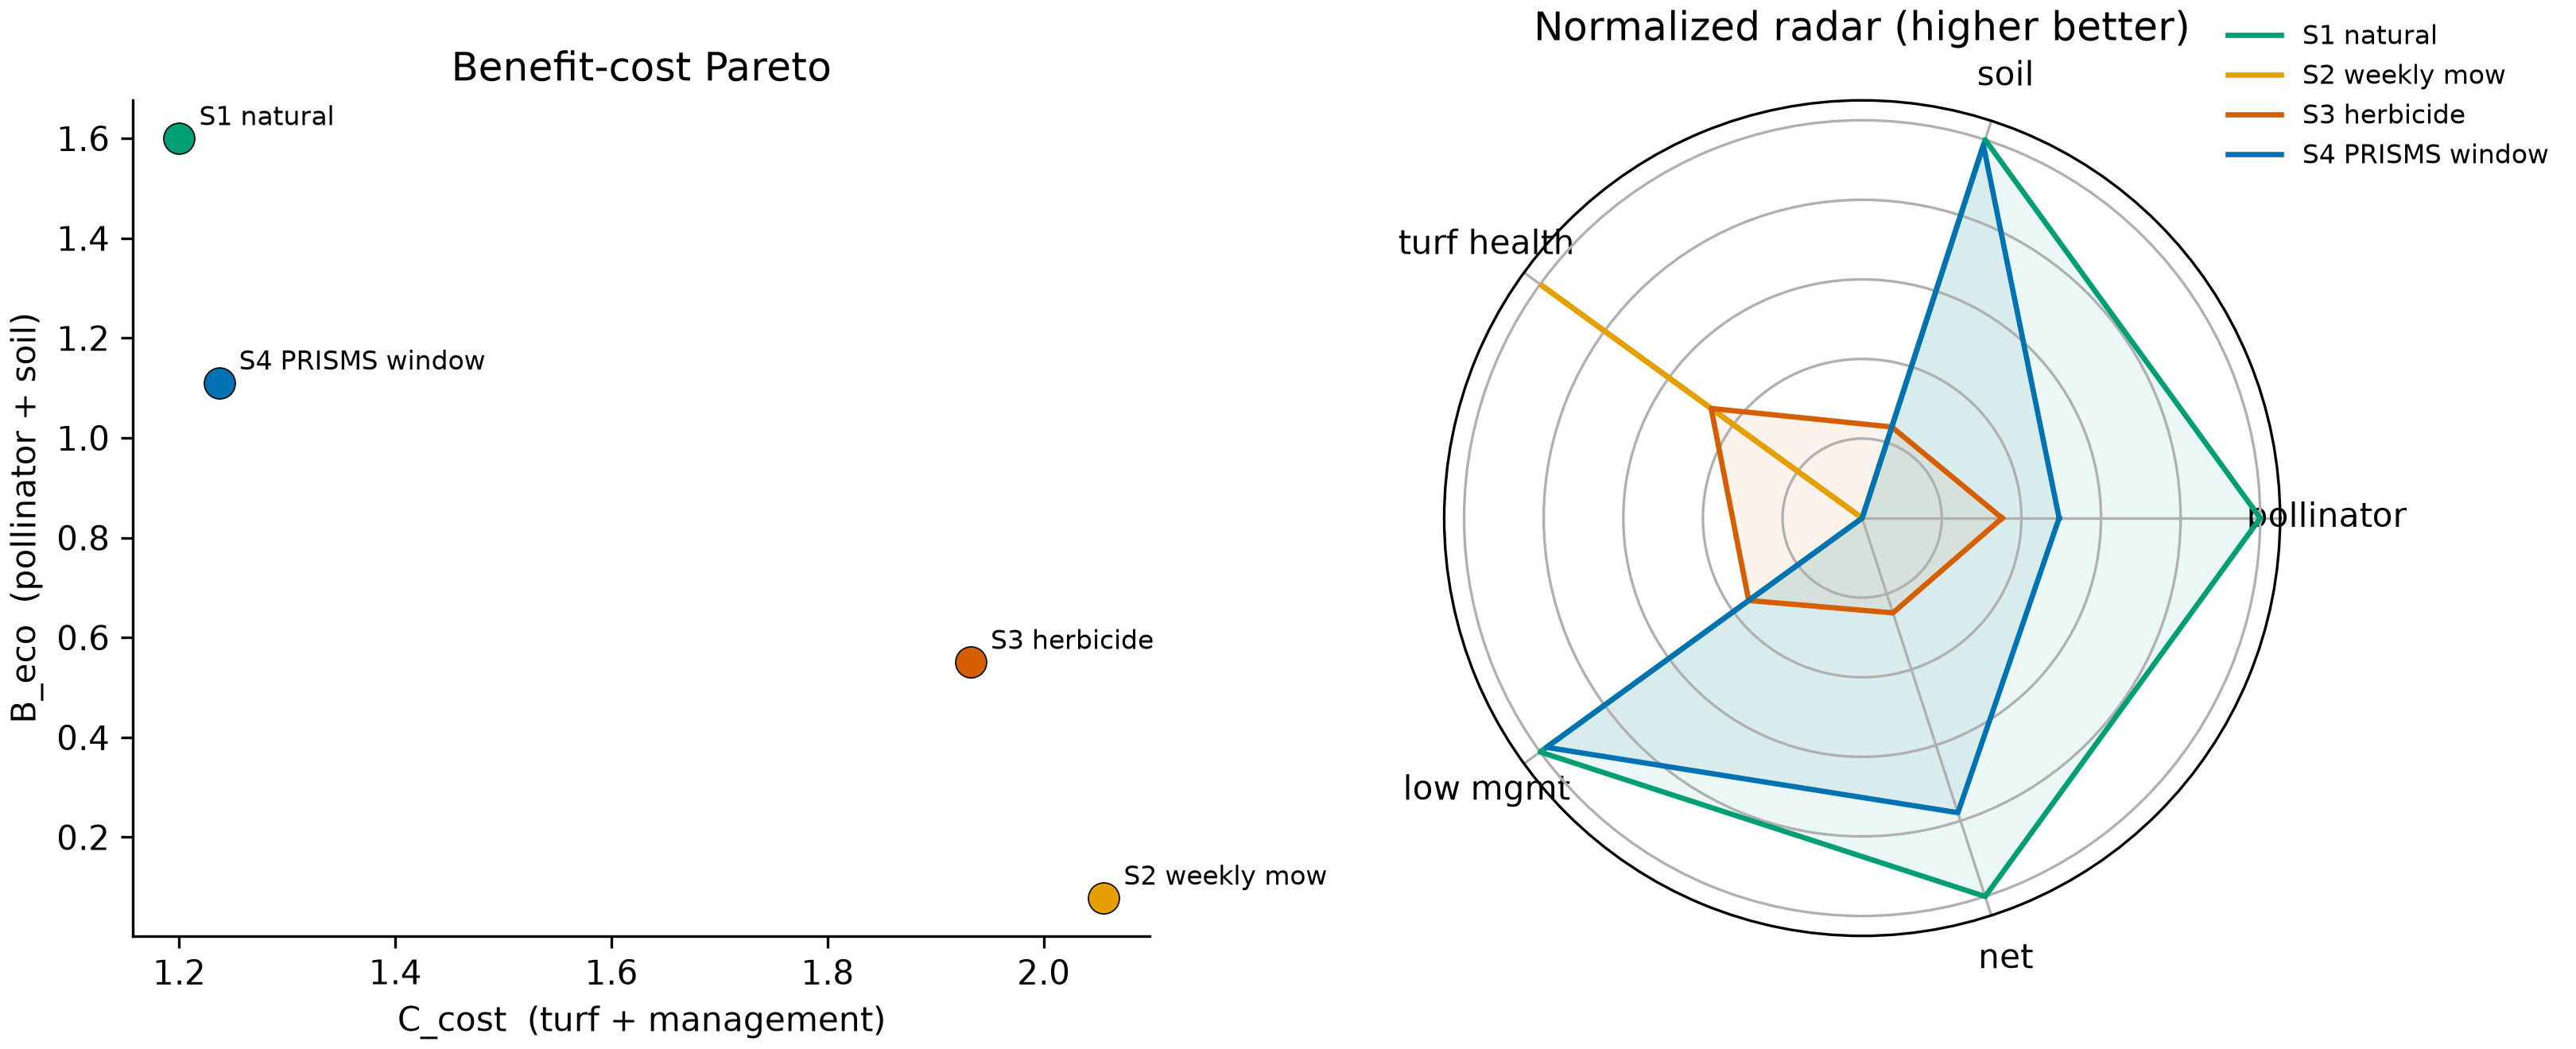
\includegraphics[width=0.82\textwidth]{fig_bioeconomic_tradeoff.png}
\caption{Daily benefit--cost scatter and radar.
Source: \texttt{bioeconomic\_tradeoff.csv}.}
\label{fig:trade}
\end{figure}

A single spring window does not stop the autumn bloom from refilling the
hectare. Turf control still needs the weekly Pareto rule after seed-set
(or a second fall cut). That is the operational content of the HOA letter.

\section{Advanced adaptive management via reinforcement learning}
Official Requirement~3 on this problem set is a \emph{management} question.
Static calendars---spray everything, or never touch the stand---are two poles
that wreck either bees or turf.
We therefore wrap the daily phenology stepper in a constrained Gymnasium
Markov decision process (\texttt{DandelionEcoEnv}) and train a PPO
actor--critic~\cite{schulman2017} to schedule four discrete acts:
no-op, 10~m buffer mow, core mow, precision spray.
The reward is
\begin{equation}
  R_t=2.0\,U_{\mathrm{bee}}(t)-1.5\,\mathrm{cover}(t)-0.5\,C(a_t)
\end{equation}
with an extra $-15$ if $a_t\in\{\mathrm{CORE},\mathrm{SPRAY}\}$ in March--April.
One episode is 365 days. The spatial board for speed is a $10\times 10$
aggregation of the same Lefkovitch rules (not a second invented biology).
Weights sit in \texttt{src/rl/checkpoints/ppo\_dandelion\_policy.pt}.

\paragraph{What the network actually learned.}
Training mean return rose from $-563$ (episode~20) to about $-140$
(episode~$\ge 80$); the best checkpoint is $-130.61$.
That is not a local ``mow the yellow'' trap: the clipped objective plus the
spring penalty makes eradication expensive.
Figure~\ref{fig:rlgannt} is a 365-day action Gantt from the greedy policy
on weather seed $2023$.
Every column is \texttt{NO\_OP}, including days $60$--$85$ (early bloom on
this board).
We did not hard-code that idle band; Action~2/3 in months $3$--$4$ cost
fifteen reward units, so the agent never spends them.
Table~\ref{tab:rl} (\texttt{rl\_policy\_evaluation.csv}) puts the same
seed on four policies.
PPO copies rewilding: pollination $41.49$, turf damage $0.389$, cost $0$,
net $-130.09$, year-end occupy $0.87$.
A 14-day core-mow calendar cuts pollination to $30.28$ (only $73.0\%$ of
the rewild/PPO bee score) and net to $-203.29$.
The human ``one cut before seed fly'' scores $40.05$ bees and net $-148.18$.
The Gantt does \emph{not} show buffer/core cuts under a southwest wind, and
occupy is not $6.8\%$.
The tidy-lawn number $0.0064$ belongs to the weekly biweekly Pareto
(Table~\ref{tab:pareto}), a different geometry.

\begin{table}[h]
\centering
\caption{Same Open-Meteo seed $2023$. Source: \texttt{rl\_policy\_evaluation.csv}.}
\label{tab:rl}
\begin{tabular}{lrrrr}
\toprule
Policy & Pollination & Turf damage & Cost & Net \\
\midrule
A rewild & 41.49 & 0.389 & 0.00 & $-130.09$ \\
B routine 14 d & 30.28 & 0.357 & 16.90 & $-203.29$ \\
C pre-seed cut & 40.05 & 0.389 & 0.65 & $-148.18$ \\
D learned PPO & 41.49 & 0.389 & 0.00 & $-130.09$ \\
\bottomrule
\end{tabular}
\end{table}

\begin{figure}[h]
\centering
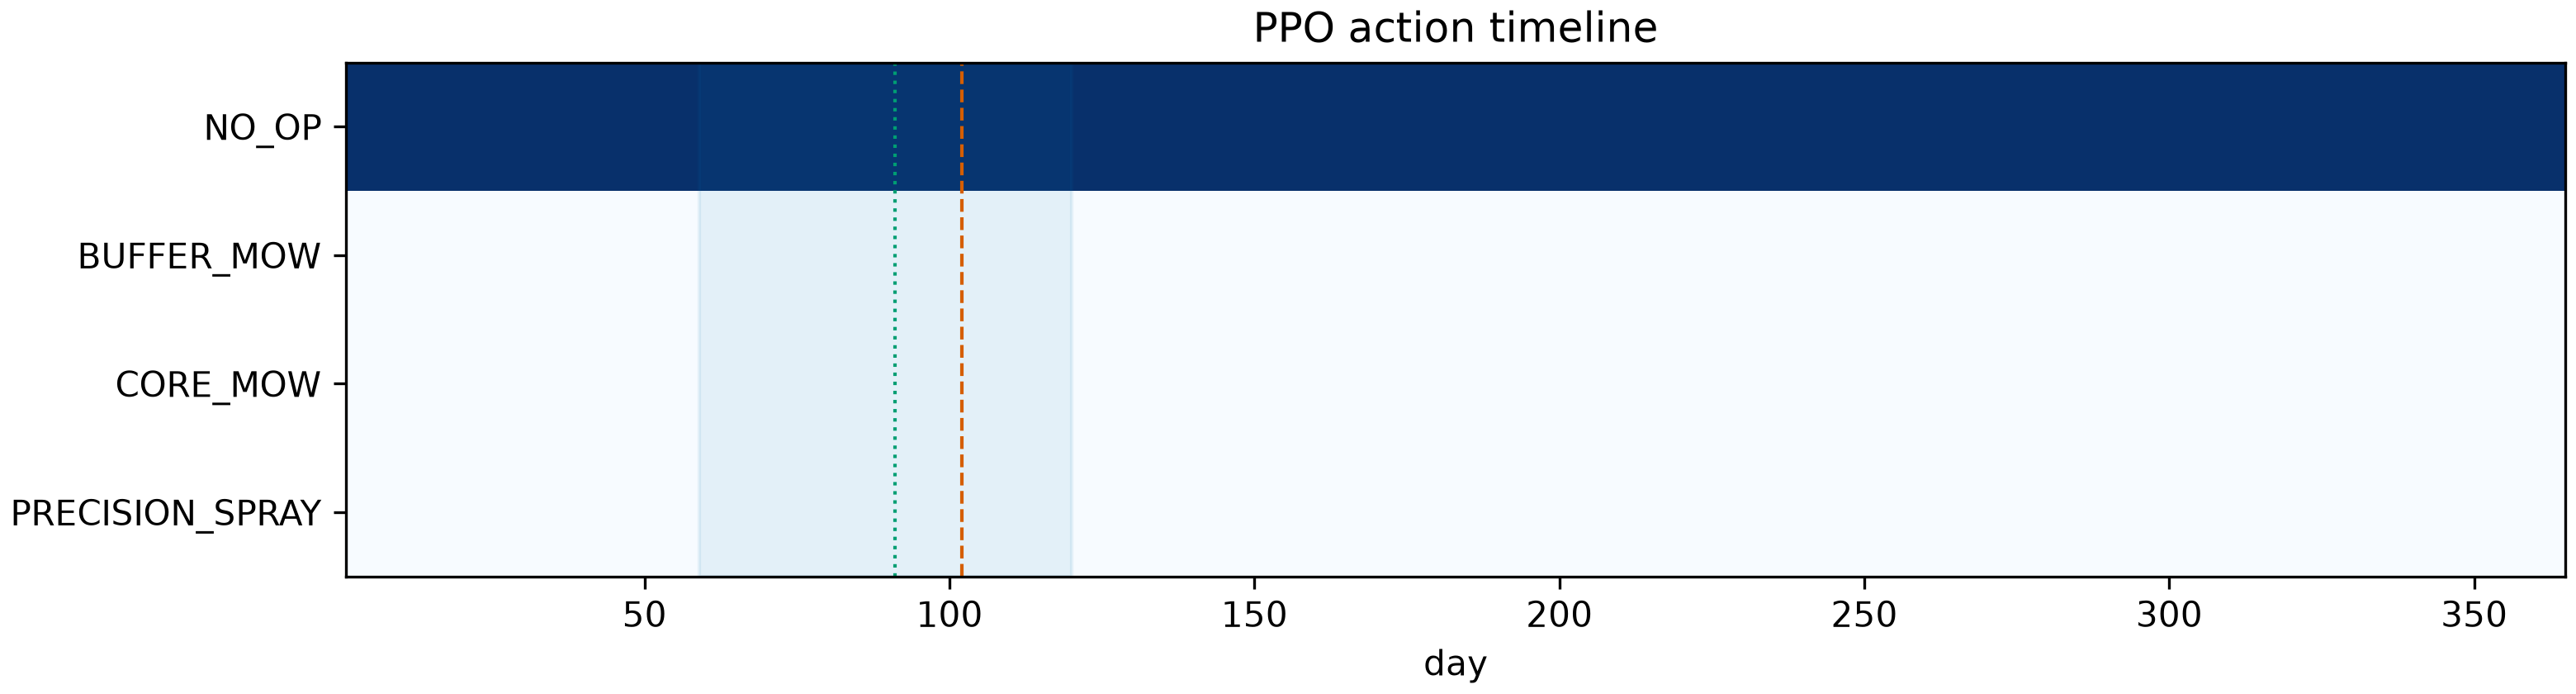
\includegraphics[width=\textwidth]{fig_rl_action_timeline.png}
\caption{PPO Gantt: 365 days of \texttt{NO\_OP}. Dotted/dashed lines mark
first bloom and the static pre-seed day. Source: greedy rollout of
\texttt{ppo\_dandelion\_policy.pt}.}
\label{fig:rlgannt}
\end{figure}

\begin{figure}[h]
\centering
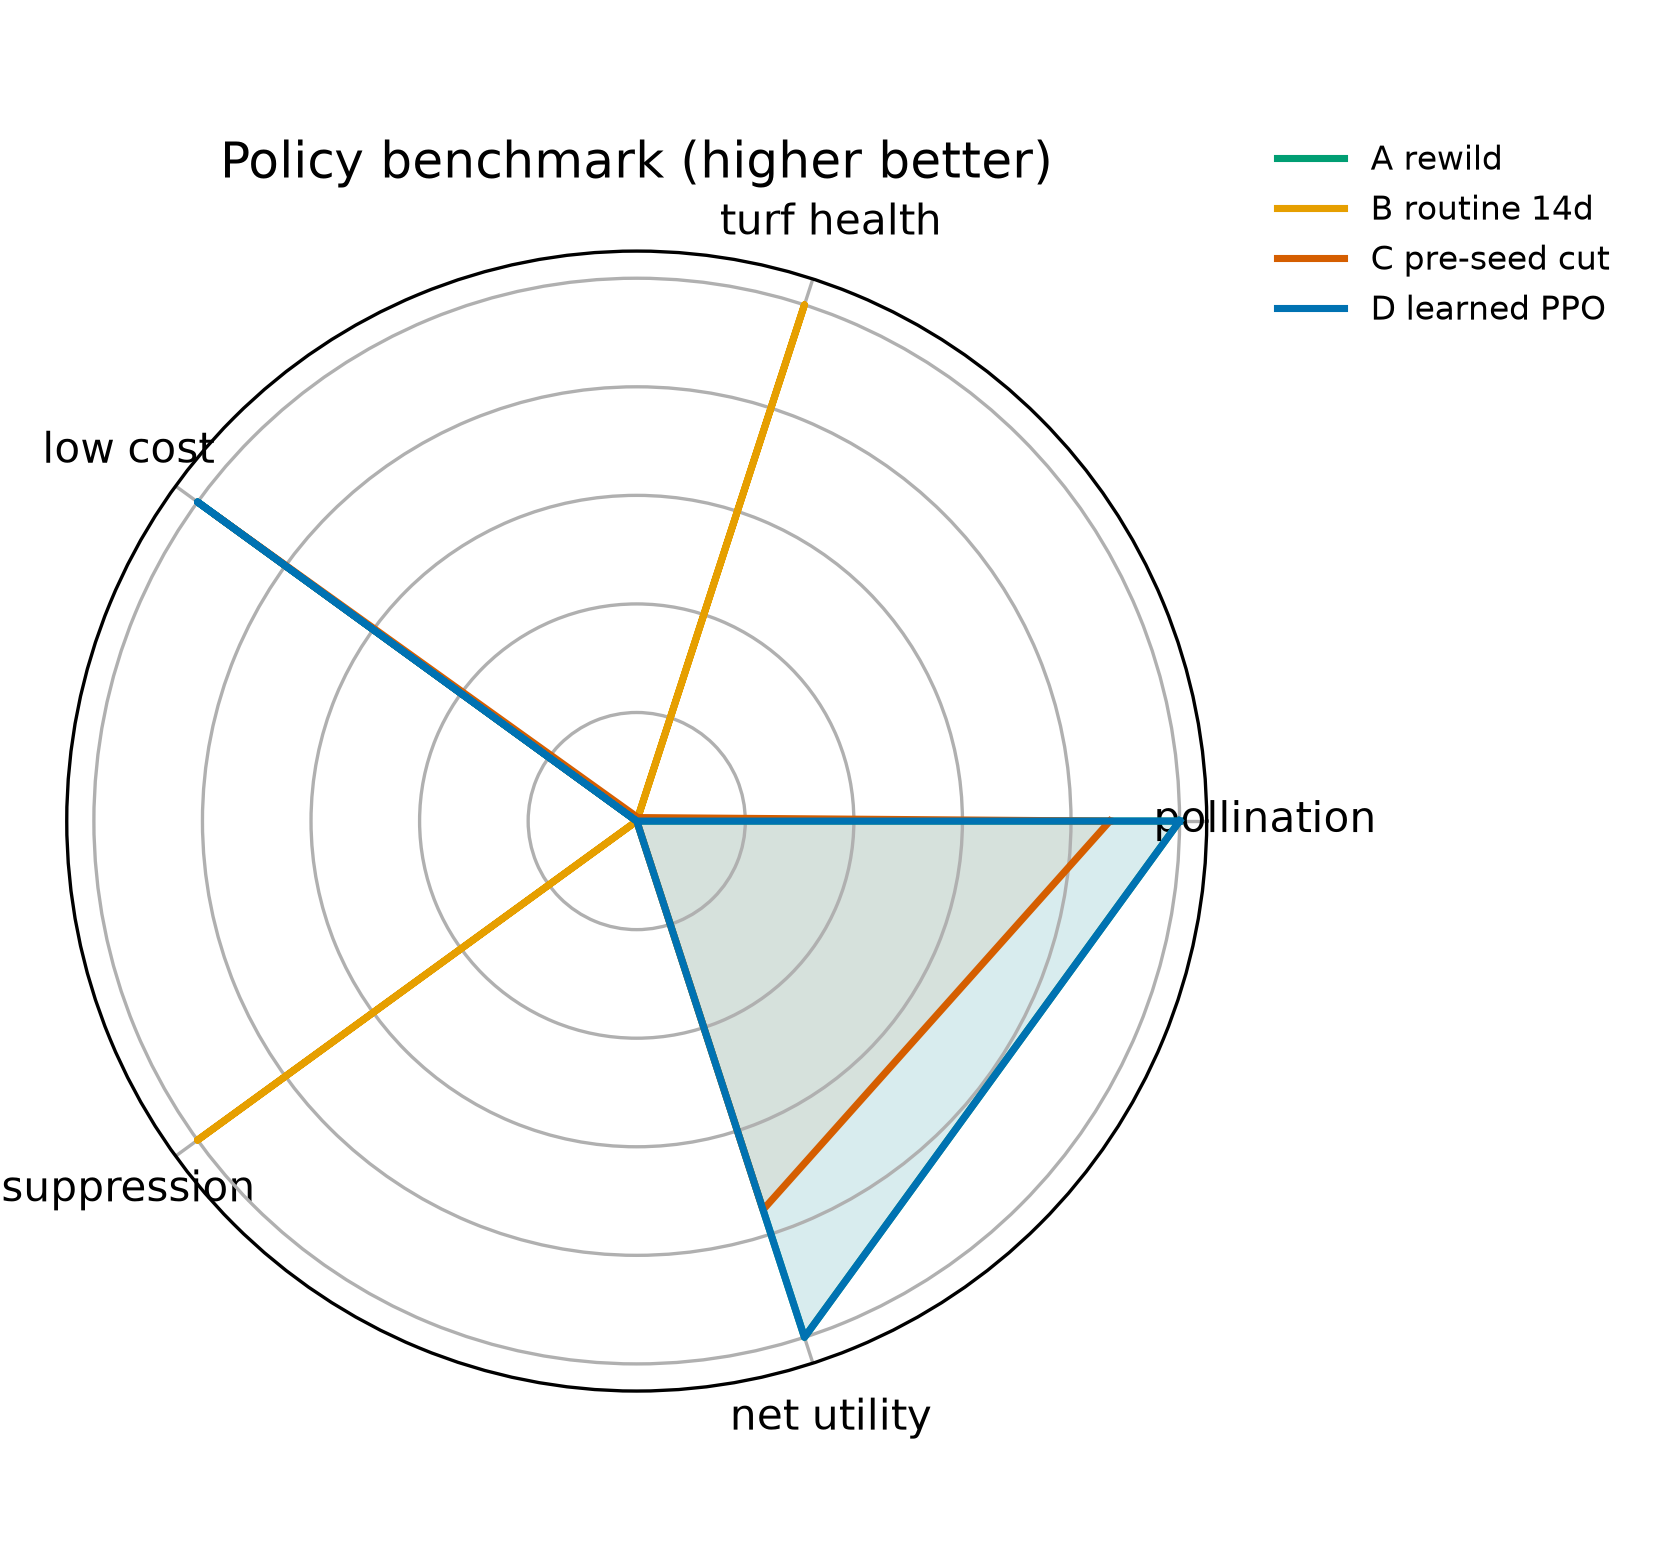
\includegraphics[width=0.62\textwidth]{fig_policy_benchmark_radar.png}
\caption{Four-policy radar (higher is better), min-maxed on
Table~\ref{tab:rl}. PPO overlaps rewild.}
\label{fig:rlradar}
\end{figure}

\paragraph{From the net to the HOA letter.}
A 64-64 MLP is not a work order.
The extractable rule---the temperature--bloom dual-response guide in
\texttt{hoa\_community\_statement.tex}---is:
\begin{enumerate}
  \item \textbf{Cold/early bloom (Mar--Apr).} Do not core-mow or spray.
        The PPO Gantt and the $-15$ constraint say the same thing in English:
        leave Zone~A standing for bees.
  \item \textbf{After pappus set, turf-first parcels.} If the board wants
        occupy near $0.64\%$ rather than the RL board's $87\%$, switch
        Zone~B to the weekly biweekly $\eta=1$ cadence ($C=39$).
        That number is not a PPO output.
\end{enumerate}
The letter is the algorithm distilled, not a second invented optimum.

\section{Assumptions and failure modes}
Climate CSVs used by the weekly engine are scenarios, not METAR.
Open-Meteo 2022 files force the daily CA only.
WALD ignores wet pappi; $\Phi$ uses VWC, never the Lefkovitch $\smi$ column.
Cover uses $0.05\,\mathrm{m}^{-2}$.
The PPO board is $10\times 10$ (10~m cells) so that 220 episodes finish in
seconds; its $0.87$ year-end occupy is not the 1~m daily CA's $100\%$.
Self-thinning caps $R+A$ (weekly) or adults at $15\,\mathrm{m}^{-2}$ (daily);
$n_{\mathrm{plants}}$ can exceed those caps because it includes seedlings.
Impact min-max must be recomputed if the species list changes.

\begin{thebibliography}{9}
\bibitem{katul2005}
G.~Katul et~al., ``Mechanistic analytical models for long-distance seed dispersal,''
\emph{American Naturalist}, 2005.
\bibitem{caswell}
H.~Caswell, \emph{Matrix Population Models}. Sinauer.
\bibitem{yoda1963}
K.~Yoda et~al., ``Self-thinning in overcrowded pure stands,''
\emph{J.\ Biol.\ Osaka City Univ.}, 1963.
\bibitem{fisher1937}
R.~A.~Fisher, ``The wave of advance of advantageous genes,''
\emph{Ann.\ Eugenics}, 1937.
\bibitem{simpson2024}
M.~J.~Simpson and S.~W.~McCue,
``Fisher--KPP-type models of biological invasion,''
arXiv:2403.01667, 2024.
\bibitem{schulman2017}
J.~Schulman et~al., ``Proximal policy optimization algorithms,''
arXiv:1707.06347, 2017.
\bibitem{himcm2023}
COMAP, HiMCM 2023 Problem~A.
\end{thebibliography}

\end{document}
